%%
% Please see http://mirror.ox.ac.uk/sites/ctan.org/macros/latex/contrib/beamer/doc/beameruserguide.pdf
%%
%\documentclass[ngerman]{beamer}
\documentclass[english,aspectratio=169]{beamer}

%\usepackage{pgfpages}
%\setbeameroption{second mode text on second screen=right}

\usepackage{mathptmx}
\usepackage[T1]{fontenc}
\usepackage[utf8]{inputenc}
\setlength{\parskip}{\smallskipamount}
\setlength{\parindent}{0pt}
\usepackage{mathtools}
\usepackage{amstext}
\usepackage{amssymb}
\usepackage{cancel}
\usepackage{stmaryrd}
\usepackage{graphicx}
\usepackage{babel}
\usepackage{isotope}
\usepackage{adjustbox}
%\usepackage{spot}
\usepackage{hyperref}

\usepackage{todo}
%\usepackage{pdfcomment}

%\usepackage{trace}

\usepackage{listings}
\usepackage{textcomp}

% Line-number = input-line-number + gaps between different line-ranges
% http://tex.stackexchange.com/a/297349/28879
\def\lst@MSkipToFirst{%
    \global\advance\lst@lineno\@ne
    \ifnum \lst@lineno=\lst@firstline
        \def\lst@next{\lst@LeaveMode \global\lst@newlines\z@
        \lst@OnceAtEOL \global\let\lst@OnceAtEOL\@empty
        \ifnum \c@lstnumber>0
            \vspace{2 mm}
        \fi
        \lst@InitLstNumber % Added to work with modified \lsthk@PreInit.
        \lsthk@InitVarsBOL
        \c@lstnumber=\numexpr-1+\lst@lineno % this enforces the displayed line numbers to always be the input line numbers
        \lst@BOLGobble}%
        \expandafter\lst@next
    \fi}
% lstinline should have same size as surrounding text:
% http://tex.stackexchange.com/a/161551/28879
\lstdefinestyle{mystyle}{
  basicstyle=%
%    \ttfamily%
%    \lst@ifdisplaystyle\scriptsize\fi
    ,
%  keywordstyle=\color{black}\bfseries,
  breaklines=true,
  showstringspaces=false
}

\lstset{%
	style=mystyle,
    mathescape=false
}

\lstdefinelanguage{posh}%
  {morekeywords={-replace},%
   sensitive=false,%
   %alsoother={$},%
   morecomment=[l]\#,%
   morecomment=[n]{\#=}{=\#},%
   morestring=[s]{"}{"},%
   morestring=[m]{'}{'},%
}[keywords,comments,strings]%

%\makeatletter
%%%%%%%%%%%%%%%%%%%%%%%%%%%%%% Textclass specific LaTeX commands.
% this default might be overridden by plain title style
%\newcommand\makebeamertitle{\frame{\maketitle}}%
% (ERT) argument for the TOC
%\AtBeginDocument{%
%  \let\origtableofcontents=\tableofcontents
%  \def\tableofcontents{\@ifnextchar[{\origtableofcontents}{\gobbletableofcontents}}
%  \def\gobbletableofcontents#1{\origtableofcontents}
%}

%%%%%%%%%%%%%%%%%%%%%%%%%%%%%% User specified LaTeX commands.

%\usetheme{Copenhagen}
%\useoutertheme{shadow}
\usetheme[hideothersubsections]{Hannover}
%\usetheme{Hannover}

%\usepackage{fontspec}

%\setsansfont{Arial}

%\setmainfont{Arial}
%\setsansfont{Fira Sans}
%\setmonofont{Fira Mono}


%\setmainfont{Museo 500}[BoldFont=Museo 700]
%\setsansfont{Museo Sans 500}
%\setmonofont{Museo Sans 500}

\setbeamercovered{transparent}

% Folienzahlen
\setbeamertemplate{footline}
{%
\begin{beamercolorbox}[wd=0.5\textwidth,ht=3ex,dp=1.5ex,leftskip=.5em,rightskip=.5em]{author in head/foot}%
\usebeamerfont{author in head/foot}%
%\insertframenumber{} / \inserttotalframenumber\hfill\insertshortauthor%
\insertframenumber{} / \insertmainframenumber{}\hfill\insertshortauthor%
\end{beamercolorbox}%
\vspace*{-4.5ex}\hspace*{0.5\textwidth}%
\begin{beamercolorbox}[wd=0.5\textwidth,ht=3ex,dp=1.5ex,left,leftskip=.5em]{title in head/foot}%
\usebeamerfont{title in head/foot}%
%\insertshorttitle%
\url{https://github.com/TheConstructor/Presentations}%
\end{beamercolorbox}%
}

% Folienzahlen 2
%\usepackage{textpos} % package for the positioning
%\addtobeamertemplate{frametitle}{}{%
%\begin{textblock*}{100mm}(\textwidth,-1\baselineskip)
%\insertframenumber{}
%\end{textblock*}}

% Keine Navigationssymbole
\setbeamertemplate{navigation symbols}{}

\setbeamertemplate{background canvas}[vertical shading][]

%\makeatother

\title[Linebreaks in T-SQL and friends]{Linebreaks in T-SQL and friends}
\author[M. Vill]{Matthias~Vill}
\institute[DM 2021]{Data Minutes 2021}
\date{11-Jun-2021}
% \titlegraphic{\includegraphics[height=0.5cm]{graphics/wwu-logo-neu}\hphantom{mm}\includegraphics[height=0.5cm]{graphics/cs_logo_nl_blue}\hphantom{mm}\includegraphics[height=0.5cm]{graphics/comsys_logo}}

%\pgfdeclareimage[height=0.5cm]{institution-logo}{graphics/comsys_logo}
%\logo{\pgfuseimage{institution-logo}}

%\AtBeginSubsection[]{%
%  \frame<beamer>{ 
%    \frametitle{Gliederung}   
%    \tableofcontents[currentsection,currentsubsection] 
%  }
%}

%\AtBeginSection[]{%
%%  \frame<beamer>{\sectionpage}
%  \frame<beamer>{ 
%    \frametitle{Agenda of \insertsection}
%    %\tableofcontents[currentsection,hideothersubsections] 
%    \tableofcontents[sectionstyle=show/hide,subsectionstyle=show/show/hide]
%  }
%}


%\beamerdefaultoverlayspecification{<+->}

\begin{document}

\frame{\maketitle}

%{
%   \usebackgroundtemplate{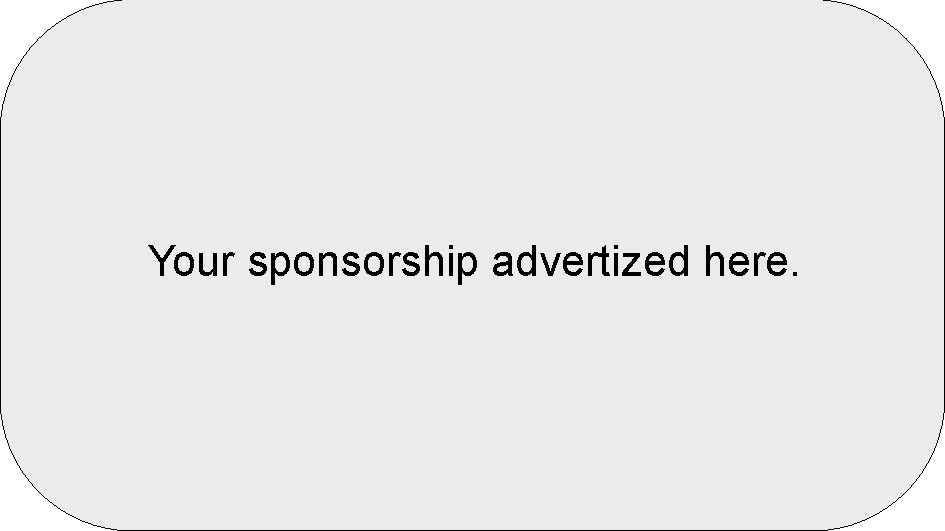
\includegraphics[height=\paperheight]{graphics/Sponsors}}
%   %\frame[plain,noframenumbering]{}
%   \frame[plain]{}
%}

\subsection*{Agenda}
\begin{frame}{Agenda}
    \tableofcontents%[hideallsubsections]
\end{frame}

\section{Overview}

\subsection{Introduction}
\begin{frame}{About me}
\begin{columns}
    \column{.75\textwidth}
        \begin{itemize}
            \item Aged 34
            \item Diplom-Informatiker ($\simeq$ Master in Computer Science)
            \item First contact with coding in the 90s (VB 3.1)
            \item First contact with Regular Expressions and (My)SQL through PHP around 2000
            \item Currently employed as Software Developer with focus on T-SQL, but also using C\# and PowerShell
            \item Experience in Java, Bash-, BAT-scripting, Ruby, \textellipsis
        \end{itemize}
        \begin{center}
            \hyperlink{https://www.youracclaim.com/badges/bd81bbb0-8416-40b7-bede-77e7f2b0d5cf}{\adjustimage{max width={1.0\columnwidth},max height={2cm},keepaspectratio}{graphics/MCSA} }
        \end{center}
    \column{.25\textwidth}
        \begin{center}
            \adjustimage{max width={1.0\columnwidth},max height={6cm},keepaspectratio}{graphics/A_054265} 
        \end{center}
    \end{columns}
\end{frame}

\section{Line Breaks}
\subsection{Introduction}
\begin{frame}{Line Breaks}

\begin{definition}
    \textbf{Newline} (frequently called \textbf{line ending}, \textbf{end of line} (\textbf{EOL}), \textbf{line feed}, or \textbf{line break}) is a \textit{control character} or \textit{sequence of control characters} in a character encoding specification (e.g. ASCII or EBCDIC) that is used to signify the end of a line of text and the start of a new one.[1] Some text editors set this special character when pressing the \smash{
\includegraphics[height=2ex]{graphics/enter-key}} key.

When displaying (or printing) a text file, this control character causes the text editor to show the following characters in a new line. 
\end{definition}

\url{https://en.wikipedia.org/wiki/Newline}
\end{frame}

\begin{frame}{Idea \& Implementation}
\begin{columns}
    \column{.60\textwidth}
        There are three common encodings of line breaks in computers:
        \begin{itemize}
            \item \texttt{character 13 (carriage-return) followed by 10 (line-feed)}\\
            \smallskip\scriptsize(Dos/Windows; \texttt{CR LF}; C-like: \texttt{\textbackslash{}r\textbackslash{}n}; PoSh: \texttt{\`{}r\`{}n})\\
            \normalsize{}Modelled after how a type-writer behaves, when you switch to a new line
            \item \texttt{character 10}\\
            \smallskip\scriptsize(Unix/Linux; \texttt{LF}; C-like: \texttt{\textbackslash{}n}; PoSh: \texttt{\`{}n})\\
            \normalsize{}Common with programmers/the web for brevity
            \item \texttt{character 13}\\
            \smallskip\scriptsize(Mac; \texttt{CR}; C-like: \texttt{\textbackslash{}r}; PoSh: \texttt{\`{}r})\\
            \normalsize{}After Mac OS X adopted the Unix standard of \texttt{LF}, this is mostly extinct
        \end{itemize}
    \column{.40\textwidth}
        \begin{center}
            \adjustimage{max width={1.0\columnwidth},max height={8cm},keepaspectratio}{graphics/typewriter}
        \end{center}
    \end{columns}
\end{frame}

\subsection{Line-Breaks in T-SQL}
\begin{frame}[fragile]{Line-Breaks in T-SQL}
\begin{itemize}
\item Preferred style: T-SQL mostly handles line-breaks just like other space characters, however some operations like \texttt{BULK INSERT} have \texttt{ROWTERMINATOR}s where \texttt{LF} or \texttt{CR LF} are default\\
    \url{https://docs.microsoft.com/en-us/sql/relational-databases/import-export/specify-field-and-row-terminators-sql-server#using-row-terminators}
\item Storing a line-break in a string
    \begin{itemize}
    \item Literal \begin{lstlisting}[language=SQL]
DECLARE @S varchar(42) = 'One
Two'
    \end{lstlisting}
    \item Explicit \begin{lstlisting}[language=SQL]
DECLARE @S varchar(42) = 'One'+CHAR(13)+CHAR(10)+'Two'
    \end{lstlisting}
    \end{itemize}
\end{itemize}
\end{frame}

\subsection{Line-Breaks in Results}
\begin{frame}[fragile]{Line-Breaks in Results}
\begin{itemize}
    \item Line-breaks will be returned in your results \& converted when using \texttt{FOR XML} or \texttt{FOR JSON}
    \item JSON: \begin{lstlisting}[language=SQL]
SELECT x='One'+CHAR(13)+CHAR(10)+'Two' FOR JSON PATH;
-- yields N'[{"x":"One\r\nTwo"}]';
    \end{lstlisting}
    \item XML: \begin{lstlisting}[language=SQL]
SELECT x='One'+CHAR(13)+CHAR(10)+'Two' FOR XML PATH;
-- yields N'<row><x>One&#x0D;'+CHAR(10)+'Two</x></row>';
    \end{lstlisting}
            \visible<2->{\texttt{CR} may cause trouble even encoded as \texttt{\&\#x0D;} see e.g. \url{https://docs.microsoft.com/en-us/dotnet/api/system.xml.xmlwritersettings.newlinehandling}}
\end{itemize}
\end{frame}

\subsection{String Escapes in T-SQL}
\begin{frame}{String Escapes in T-SQL}
\begin{columns}
    \column{.60\textwidth}
        \begin{itemize}
            \item Generally all characters are taken as they are (within the collation)
            \item To get one \lstinline[language=SQL]{'} write \lstinline[language=SQL]{''}
            \item There is however 'Line Continuation' \only<1>{\lstinputlisting[language=SQL,linerange=1-5]{demos/line-continuation.sql}}\only<2>{\lstinputlisting[language=SQL,linerange=1-6]{demos/line-continuation.sql}}
        \end{itemize}
    \column{.40\textwidth}
        \begin{center}
            \adjustimage{max width={1.0\columnwidth},max height={7cm},keepaspectratio}{graphics/lighthouse}%
        \end{center}
    \end{columns}
\end{frame}

\subsection{Escaping line-continuation}
\begin{frame}{Escaping line-continuation}
\begin{itemize}
    \item \url{https://docs.microsoft.com/en-us/sql/t-sql/language-elements/sql-server-utilities-statements-backslash} \textbf{does not list any escapes for line-continuation}
    \item But you can do this \lstinputlisting[language=SQL,linerange=9-14]{demos/line-continuation.sql}
\end{itemize}
\end{frame}

\subsection[SSMS]{SQL Management Studio}
\begin{frame}{SQL Management Studio}
\begin{columns}
    \column{.60\textwidth}
        \begin{itemize}
        \item<1| only@1> SSMS will \textbf{by default} discard line-breaks in grid-results!
        \item<2-> There is one setting to change it for the current session/tab (\texttt{Query} \textrightarrow{} \texttt{Query Options…})\only<2>{\\\adjustimage{max width={1.0\columnwidth},max height={4cm},keepaspectratio}{graphics/menu_query_query_options}}
        \item<3-> and \textbf{another} to change it for new sessions (\texttt{Tools} \textrightarrow{} \texttt{Options})\only<3>{\\\adjustimage{max width={0.9\columnwidth},max height={4cm},keepaspectratio}{graphics/menu_tools_options}}
        \end{itemize}
    \column{.40\textwidth}
        \begin{center}
            \only<2->{\adjustimage{max width={1.0\columnwidth},max height={4cm},keepaspectratio}{graphics/query_options}}
            \only<3->{\adjustimage{max width={1.0\columnwidth},max height={4cm},keepaspectratio}{graphics/options}}
        \end{center}
    \end{columns}
\end{frame}

\subsection[ADS]{Azure Data Studio}
\begin{frame}{Azure Data Studio}
    Under Settings go to \texttt{Data} \textrightarrow{} \texttt{Query Editor} \textrightarrow{} \texttt{Results: Copy Remove New Line} (queryEditor.results.copyRemoveNewLine); immediately takes effect

    \begin{center}
        \adjustimage{max width={1.0\columnwidth},max height={5cm},keepaspectratio}{graphics/ads_options}
    \end{center}
\end{frame}

\section{Summary}

%\subsection*{Summary}
\begin{frame}{Summary}
\begin{columns}
    \column{.60\textwidth}
    \begin{itemize}
        \item Most people think line-breaks 'just work'
        \item Most people think they only ever need to take care of quotes in T-SQL-strings
        \item Reality is at it again and makes it a bit more complicated
    \end{itemize}
    \column{.40\textwidth}
        \begin{center}
            \adjustimage{max width={1.0\columnwidth},max height={8cm},keepaspectratio}{graphics/quirks}
            \tiny(Author unknown)
        \end{center}
\end{columns}
\end{frame}

\appendix
% Folienzahlen
\setbeamertemplate{footline}
{%
\begin{beamercolorbox}[wd=0.5\textwidth,ht=3ex,dp=1.5ex,leftskip=.5em,rightskip=.5em]{author in head/foot}%
\usebeamerfont{author in head/foot}%
%\insertframenumber{} / \inserttotalframenumber\hfill\insertshortauthor%
\insertframenumber{} / \insertmainframenumber{} + \insertappendixframenumber{}\hfill\insertshortauthor%
\end{beamercolorbox}%
\vspace*{-4.5ex}\hspace*{0.5\textwidth}%
\begin{beamercolorbox}[wd=0.5\textwidth,ht=3ex,dp=1.5ex,left,leftskip=.5em]{title in head/foot}%
\usebeamerfont{title in head/foot}%
\insertshorttitle%
\end{beamercolorbox}%
}
\beamerdefaultoverlayspecification{}

\section*{Apendix}

\subsection*{Feedback}
\begin{frame}{Feedback}
\begin{center}
{\usebeamerfont*{title} \usebeamercolor[fg]{title} Please provide feedback}
\end{center}
\end{frame}

\end{document}

